
\section{ Yingyu Wu's Computational Experience}
Normally, I use R to simulate data. Latex is also useful to write a paper.\par
Last semester, I used the research methods of Ridge regression and Lasso regression to explore the influencing factors of China’s fiscal revenue. I transfered the original data from the database into .csv fomat, and then used R to open it. After analyzing data, I conducted a simulation study by using R. Then used boxplot to compare the two regression models.\par

I don't have much experience about programming, I'm looking forward to gain more knowledge and experience in this course.\par

\subsection{Formula}
Some formula I used in my paper:
\begin{equation}
y=\beta_1x_1+\beta_2x_2+\cdots+\beta_ix_i+\varepsilon
\end{equation}
\begin{equation}
\begin{cases}
min\|y-X\omega\Vert_2^2+\lambda\|\omega\Vert_2^2 \\
s.t.\quad\|\omega\Vert_2^2=\sqrt {\sum_i x_i^2}\\
\lambda>0
\end{cases}
\end{equation}
\begin{equation}
J(\omega)=\sum\limits_{i=1}^m (y_i-\sum\limits_{j=0}^p \omega_jx_ij)^2 + \lambda \sum\limits_{j=1}^p \omega_j^2
\end{equation}
\begin{equation}
J(\omega)=\sum\limits_{i=1}^m (y_i-\sum\limits_{j=0}^p \omega_jx_ij)^2 + \lambda \sum\limits_{j=1}^p |\omega_j^2\vert
\end{equation}
\begin{equation}
\hat{\beta}_L=arg min(Y-X\beta)(Y-X\beta)'+\lambda\|\beta\Vert_1
\end{equation}

\subsection{Table}
The table of the coefficient value of ridge regression and lasso regression:\par
\begin{table}[H]
\caption{\textbf{the coefficient value of ridge regression and lasso regression:}}
\centering
\begin{tabular}{@{}cccccc@{}}
\toprule
\multirow{2}{*}{Variables} & Coefficient  & Coefficient & \multirow{2}{*}{Variables} & Coefficient & Coefficient  \\ 
& of Ridge     & of Lasso & & of Ridge & of Lasso \\
\midrule
$X_1$      & 0.06809683           & 0                    & $X_9$        & 0.1151936            & 0.1684967            \\
$X_2$        & 0.1241104            & 0.3147499            & $X_{10}$       & 0.07165713           & 0.04643967           \\
$X_3$        & 0.06691223          & 0                    & $X_{11}$       & 0.0452909            & 0                    \\
$X_4$        & 0.05347575           & 0                    & $X_{12}$       & 0.048277055          & 0.000234869          \\
$X_5$        & 0.09041124           & 0                    & $X_{13}$       & 0.1026359            & 0.1507419            \\
$X_6$        & 0.150904             & 0.2335954            & $X_{14}$       & 0.06882711           & 0                    \\
$X_7$        & 0.1425961            & 0.1915404            & $X_{15}$       & 0.0674552            & 0                    \\
$X_8$        & 0.02842502           & 0                    & $X_{16}$       & 0.1289195            & 0.1085074  \\       
\bottomrule
\end{tabular}
\end{table}
\subsection{images}
These are some reslut images I generate with R.\par
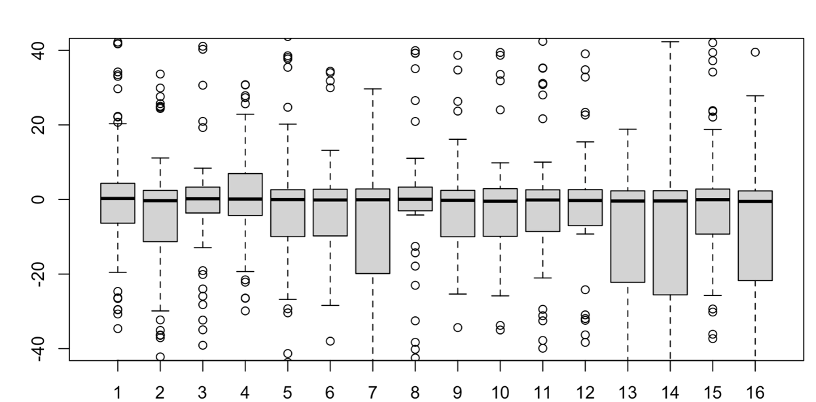
\includegraphics[width = 0.9\textwidth]{figure1.jpg}\par
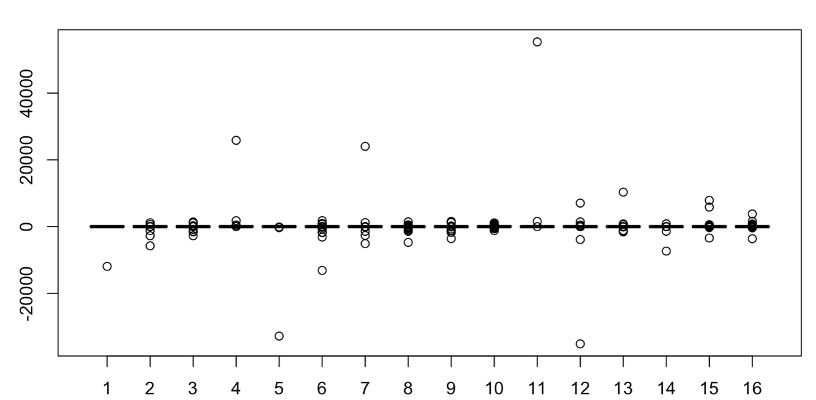
\includegraphics[width = 0.9\textwidth]{figure2.jpg}\par
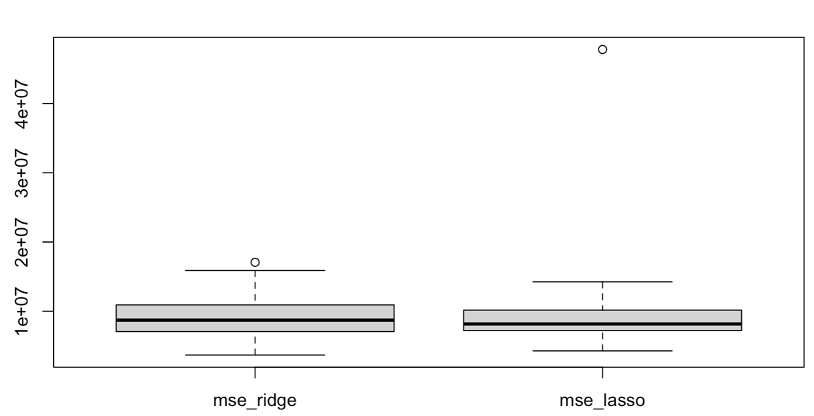
\includegraphics[width = 0.9\textwidth]{figure3.jpg}\par
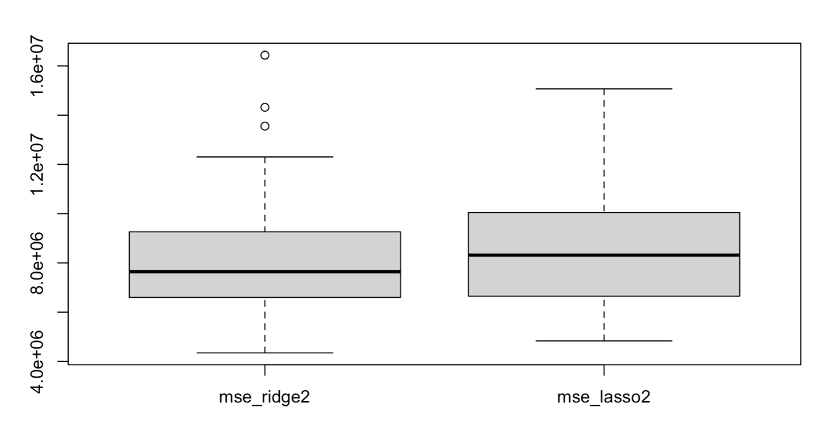
\includegraphics[width = 0.9\textwidth]{figure4.jpg}\par

